\documentclass[11pt,a4paper]{article}
\usepackage[margin=2.2cm]{geometry}
\usepackage{parskip}
\setlength{\parskip}{4pt}
\usepackage[T1]{fontenc}
\usepackage[utf8]{inputenc}
\usepackage{mathptmx}
\usepackage{textcomp}
\usepackage{microtype}
\usepackage{amsmath,amssymb}
\usepackage{graphicx}
\usepackage{xcolor}
\usepackage{booktabs}
\usepackage{tabularx}
\usepackage{array}
\usepackage{url}
\usepackage{enumitem}
\usepackage{tikz}
\usetikzlibrary{shapes.geometric, arrows.meta, positioning, fit, calc}
\usepackage{caption}
\usepackage{subcaption}
\usepackage{placeins}
\usepackage{needspace}
\usepackage{float}
\usepackage{pdflscape}
\usepackage{listings}
\usepackage[hidelinks]{hyperref}
\urlstyle{same}
\graphicspath{{../../report/figures/}{./}}
\captionsetup{font=footnotesize,labelfont=bf}
\setlength{\textfloatsep}{8pt plus 2pt minus 2pt}
\setlength{\intextsep}{8pt plus 2pt minus 2pt}
\setlist{nosep,leftmargin=1.3em}
\newcommand{\vfour}{v4}
\newcommand{\ubrk}{\textunderscore\allowbreak}
\DeclareRobustCommand{\code}[1]{{\ttfamily\small\let\_\ubrk #1}}
\newcolumntype{L}[1]{>{\raggedright\arraybackslash}p{#1}}
\newcolumntype{Y}{>{\raggedright\arraybackslash}X}
\lstset{basicstyle=\ttfamily\footnotesize,breaklines=true,frame=single,framerule=0.3pt,rulecolor=\color{black!40},xleftmargin=2pt,xrightmargin=2pt,columns=fullflexible,keepspaces=true,showstringspaces=false}

% shared TikZ styles
\tikzset{
  bx/.style={rectangle,rounded corners=3pt,draw=black!60,fill=blue!8,align=center,font=\footnotesize,inner sep=3pt},
  gx/.style={rectangle,rounded corners=3pt,draw=black!60,fill=green!10,align=center,font=\footnotesize,inner sep=3pt},
  ox/.style={rectangle,rounded corners=3pt,draw=black!60,fill=orange!14,align=center,font=\footnotesize,inner sep=3pt},
  rx/.style={rectangle,rounded corners=3pt,draw=black!60,fill=red!8,align=center,font=\footnotesize,inner sep=3pt},
  gy/.style={rectangle,rounded corners=3pt,draw=black!50,fill=black!5,align=center,font=\footnotesize,inner sep=3pt},
  dm/.style={diamond,aspect=2.4,draw=black!60,fill=orange!14,align=center,font=\footnotesize,inner sep=1pt},
  ar/.style={-{Stealth[length=2mm]},thick,draw=black!65},
  lb/.style={font=\scriptsize,text=black!75,inner sep=1.2pt}
}

\begin{document}

\begin{center}
{\LARGE\bfseries AsanaAI: System and Model Architecture}\\[6pt]
{\large Technical design document}\\[10pt]
Anamitra Sarkar \quad Debjit Deb Barman \quad Adrija Ray Mondal \quad Tanima Samanta\\[3pt]
Supervisor: Mr.\ Sujit Chakraborty, Assistant Professor, Department of CSE (AI/ML)\\[2pt]
RCC Institute of Information Technology, Kolkata, West Bengal, India\\[2pt]
Final-year project P05
\end{center}
\vspace{4pt}
\hrule
\vspace{6pt}

\noindent\textbf{Scope.} This document describes how AsanaAI is built: its components, the path of one camera frame through the system, the three trained models and the rule engine, and how everything is deployed. It contains no accuracy results; those are in the research paper and the project report. Live app: \url{https://yoga-posture-correction-system.vercel.app}. API: \url{https://arko007-yoga-pose.hf.space}.

\tableofcontents
\clearpage

%==========================================================================
\section{System Overview}
AsanaAI is a yoga coach that watches a person through a camera, names the pose they are in, scores their form, and tells them in English, Hindi or Bengali what to adjust, on screen and aloud. It runs as a web app (a progressive web app that can be installed on a phone) backed by a small CPU server. The central design choice is that the camera image never leaves the device: the browser turns each frame into 33 body landmarks, and only numbers derived from them are sent to the server. Figure~\ref{fig:arch} (on its own page after Section~2) shows the whole data flow, and Table~\ref{tab:components} lists the components.

\begin{table}[ht]
\centering\small
\caption{Components, where they run and what they do.}\label{tab:components}
\begin{tabularx}{\textwidth}{@{}L{3.2cm}L{3.0cm}Y@{}}
\toprule
Component & Runs on & Role \\ \midrule
Web app & Browser (Next.js 14, React 18, next-pwa service worker) & Camera, pose engine, joint angles, skeleton buffer, interface, speech, local storage of the user's calibration profile \\
Pose engine & Browser (GPU, or CPU in a Web Worker, or WASM) & Image $\to$ 33 landmarks $(x,y,z,v)$ \\
On-device coach (basic mode) & Browser (TypeScript) & Port of the rule engine and coaching templates; used when the server is unreachable \\
Android app & Capacitor 8 wrapper (plus an Expo companion app) & Packages the same web app for Android \\
API server & Hugging Face Space (FastAPI, PyTorch, CPU) & Frame analysis, sequence analysis, coaching text \\
Pose MLPs (namer, gate) & Server & Name the pose; veto ``not one of my poses''; form score \\
ST-GCN & Server & Second opinion from 60 frames of skeleton motion \\
Rule engine & Server (and browser) & Per-joint deviations from reference angle bands \\
Coaching service & Server (calls an external language model) & Template $\to$ optional paraphrase $\to$ safety screen \\
Model repository & Hugging Face Hub & Stores weights and class encoders; the server downloads them at start-up \\ \bottomrule
\end{tabularx}
\end{table}


%==========================================================================
\section{Design Principles}
\begin{enumerate}
\item \textbf{Privacy by construction.} The request carries 15 joint angles, or 60 frames of landmark coordinates, never pixels. There is no code path that uploads an image.
\item \textbf{Small models on a CPU.} The two pose MLPs have 0.36\,M parameters each and the ST-GCN 0.89\,M; all three weight files together are 6.6\,MB. The server needs no GPU.
\item \textbf{Abstain rather than guess.} A second model can veto a pose name (``not one of my poses''); joints the camera cannot see are neither scored nor coached; the sequence model only speaks when it is confident.
\item \textbf{Graceful degradation.} Every layer has a fallback: three pose engines, an on-device coach when the server is asleep, the original decision path if the gate model fails to load, and a reviewed template if the language model is unavailable or produces an unsafe sentence.
\item \textbf{Roles for each component.} Neural networks name the pose and judge form; the rule engine supplies per-joint corrections because they are defined by reference angle bands; the language model may only rewrite a reviewed sentence.
\end{enumerate}

\begin{landscape}
\thispagestyle{empty}
\begin{figure}[p]
\centering
\resizebox{24.5cm}{!}{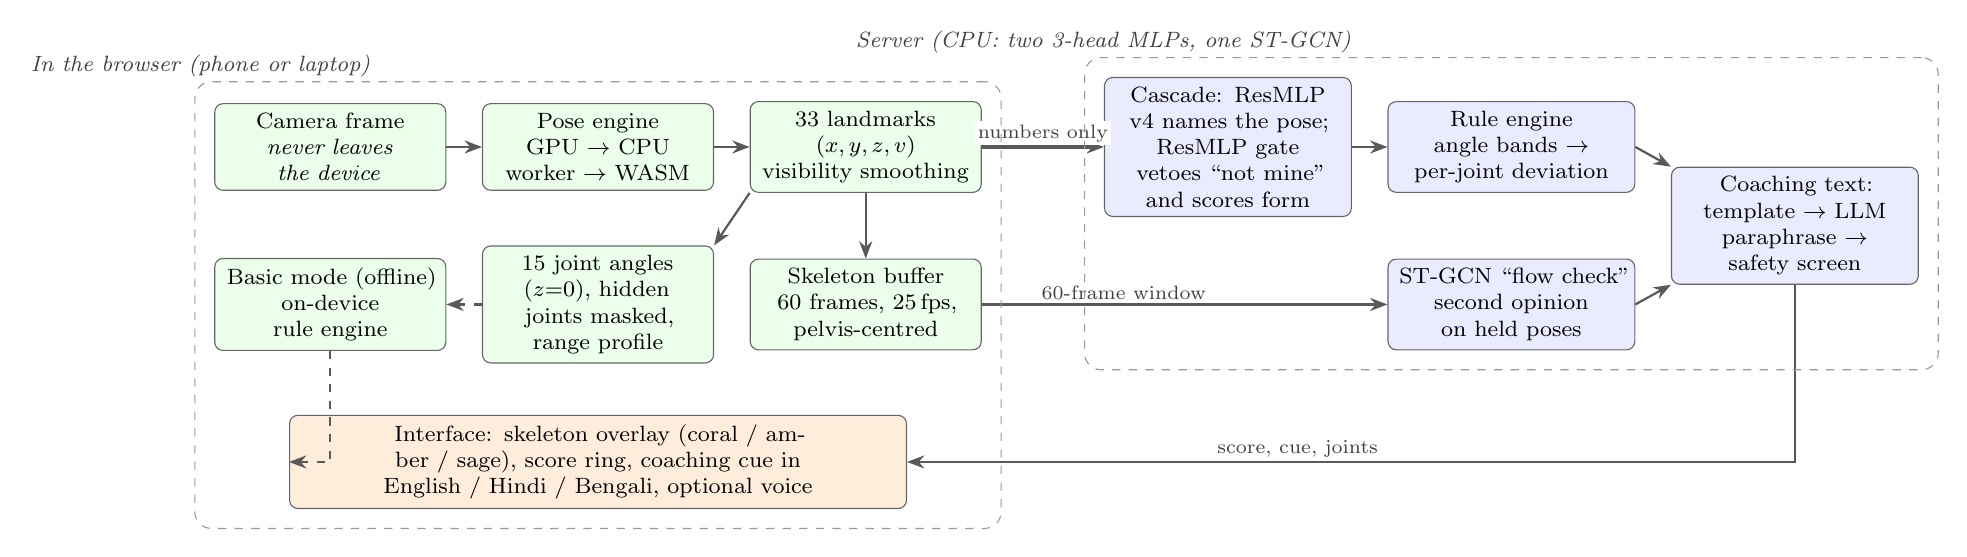
\begin{tikzpicture}[node distance=0pt, x=1cm, y=1cm]
\tikzset{
  dev/.style={rectangle,rounded corners=3pt,draw=black!60,fill=green!8,text width=2.7cm,align=center,minimum height=1.1cm,font=\footnotesize},
  srv/.style={rectangle,rounded corners=3pt,draw=black!60,fill=blue!8,text width=2.9cm,align=center,minimum height=1.1cm,font=\footnotesize},
  ui/.style={rectangle,rounded corners=3pt,draw=black!60,fill=orange!14,text width=7.6cm,align=center,minimum height=1.1cm,font=\footnotesize},
  ar/.style={-{Stealth[length=2.2mm]},thick,draw=black!65},
  lab/.style={font=\scriptsize,text=black!75,inner sep=1.2pt,fill=white},
  zone/.style={rectangle,rounded corners=6pt,draw=black!40,dashed,inner sep=7pt}
}
% ---- in the browser
\node[dev] (cam) at (0,0)    {Camera frame\\ \textit{never leaves the device}};
\node[dev] (eng) at (3.4,0)  {Pose engine\\ GPU $\rightarrow$ CPU worker $\rightarrow$ WASM};
\node[dev] (lm)  at (6.8,0)  {33 landmarks $(x,y,z,v)$\\ visibility smoothing};
\node[dev] (loc) at (0,-2.0) {Basic mode (offline)\\ on-device rule engine};
\node[dev] (ang) at (3.4,-2.0) {15 joint angles ($z{=}0$), hidden joints masked, range profile};
\node[dev] (buf) at (6.8,-2.0) {Skeleton buffer\\ 60 frames, 25\,fps, pelvis-centred};
\node[ui]  (uin) at (3.4,-4.0) {Interface: skeleton overlay (coral / amber / sage), score ring, coaching cue in English / Hindi / Bengali, optional voice};
% ---- on the server
\node[srv] (cas) at (11.4,0)    {Cascade: ResMLP \vfour{} names the pose; ResMLP gate vetoes ``not mine'' and scores form};
\node[srv] (rul) at (15.0,0)    {Rule engine\\ angle bands $\rightarrow$ per-joint deviation};
\node[srv] (stg) at (15.0,-2.0) {ST-GCN ``flow check''\\ second opinion on held poses};
\node[srv] (coa) at (18.6,-1.0) {Coaching text: template $\rightarrow$ LLM paraphrase $\rightarrow$ safety screen};
% ---- arrows
\draw[ar] (cam)--(eng); \draw[ar] (eng)--(lm);
\draw[ar] (lm.south west)--(ang.north east);
\draw[ar] (lm.south)--(buf.north);
\draw[ar,dashed] (ang.west)--(loc.east);
\draw[ar,line width=1.2pt] (lm.east)-- node[above,lab]{numbers only} (cas.west);
\draw[ar,line width=1.2pt] (buf.east)-- node[above,lab,pos=0.35]{60-frame window} (stg.west);
\draw[ar] (cas)--(rul);
\draw[ar] (rul.east)--(coa.north west);
\draw[ar] (stg.east)--(coa.south west);
\draw[ar] (coa.south) |- node[above,lab,pos=0.78]{score, cue, joints} (uin.east);
\draw[ar,dashed] (loc.south) |- (uin.west);
% ---- zones
\node[zone,fit=(cam)(eng)(lm)(loc)(ang)(buf)(uin),label={[lab,font=\footnotesize\itshape]above left:In the browser (phone or laptop)}] {};
\node[zone,fit=(cas)(rul)(stg)(coa),label={[lab,font=\footnotesize\itshape]above left:Server (CPU: two 3-head MLPs, one ST-GCN)}] {};
\end{tikzpicture}
}
\caption{End-to-end architecture. Everything on the left runs in the browser: the camera frame is converted to 33 landmarks by a pose engine chosen automatically, hidden joints are masked, and only numbers are sent. The server holds three small neural networks and a rule engine. Dashed arrows show the offline path, in which an on-device port of the rule engine keeps a basic mode working.}
\label{fig:arch}
\end{figure}
\end{landscape}

%==========================================================================
\section{Client Architecture (in the Browser)}
\subsection{The path of one frame}
\begin{figure}[ht]
\centering
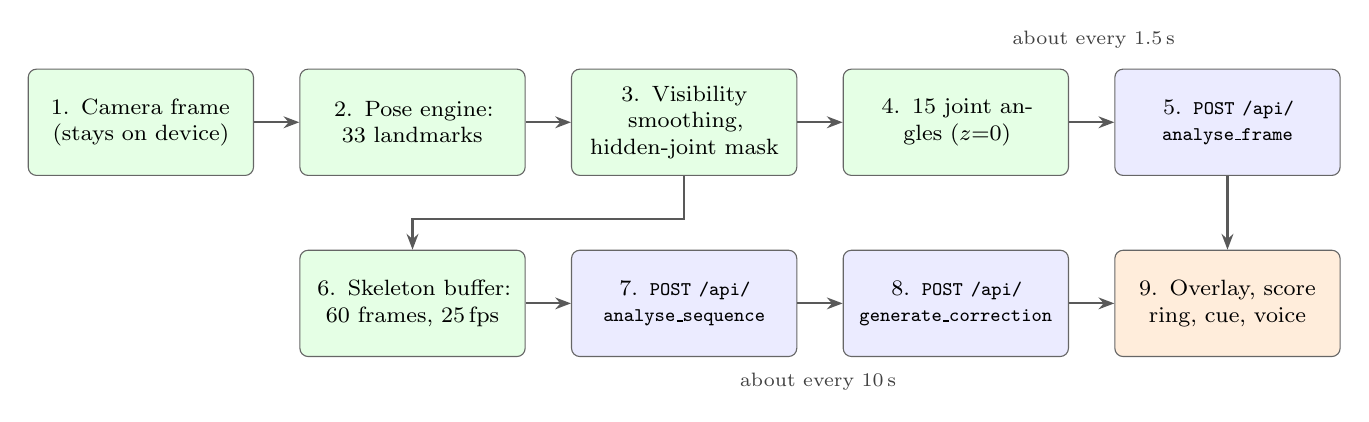
\begin{tikzpicture}[x=1cm,y=1cm]
\tikzset{nd/.style={minimum height=1.35cm,text width=2.65cm}}
\node[gx,nd] (a) at (0,0) {1. Camera frame\\ (stays on device)};
\node[gx,nd] (b) at (3.45,0) {2. Pose engine:\\ 33 landmarks};
\node[gx,nd] (c) at (6.9,0) {3. Visibility smoothing, hidden-joint mask};
\node[gx,nd] (d) at (10.35,0) {4. 15 joint angles ($z{=}0$)};
\node[bx,nd] (e) at (13.8,0) {5. \scriptsize\texttt{POST /api/}\\ \scriptsize\texttt{analyse\_frame}};
\node[gx,nd] (f) at (3.45,-2.3) {6. Skeleton buffer:\\ 60 frames, 25\,fps};
\node[bx,nd] (g) at (6.9,-2.3) {7. \scriptsize\texttt{POST /api/}\\ \scriptsize\texttt{analyse\_sequence}};
\node[bx,nd] (h) at (10.35,-2.3) {8. \scriptsize\texttt{POST /api/}\\ \scriptsize\texttt{generate\_correction}};
\node[ox,nd] (i) at (13.8,-2.3) {9. Overlay, score ring, cue, voice};
\foreach \s/\t in {a/b,b/c,c/d,d/e}{\draw[ar] (\s)--(\t);}
\draw[ar] (c.south) -- ++(0,-0.55) -| (f.north);
\draw[ar] (f)--(g); \draw[ar] (g)--(h); \draw[ar] (h)--(i);
\draw[ar] (e.south) -- (i.north);
\node[lb] at (12.1,1.05) {about every 1.5\,s};
\node[lb] at (8.6,-3.3) {about every 10\,s};
\end{tikzpicture}
\caption{The client pipeline. Steps 1--4, 6 and 9 run on the device (green and orange); 5, 7 and 8 are the three network calls to the server (blue).}
\end{figure}

\subsection{Pose engine and its fallback ladder}
The pose engine returns 33 MediaPipe landmarks per frame, each as $(x,y,z,v)$ where $v$ is the estimator's visibility. Different phones can break different engines (a GPU driver can crash MediaPipe), so the app picks one automatically (Figure~\ref{fig:ladder}). The decision is remembered per browser version and is invisible to the user.

\begin{figure}[ht]
\centering
\resizebox{0.5\textwidth}{!}{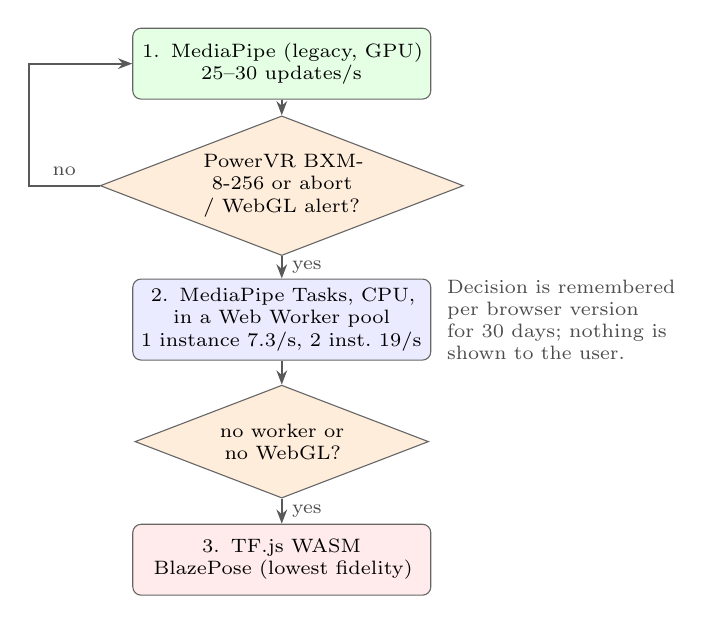
\begin{tikzpicture}[x=1cm,y=1cm]
\tikzset{
  nb/.style={rectangle,rounded corners=3pt,draw=black!60,fill=blue!8,text width=3.55cm,align=center,minimum height=0.9cm,font=\scriptsize},
  nd/.style={diamond,aspect=2.6,draw=black!60,fill=orange!14,text width=2.3cm,align=center,inner sep=1pt,font=\scriptsize},
  ar/.style={-{Stealth[length=1.8mm]},thick,draw=black!65},
  lb/.style={font=\scriptsize,text=black!70}
}
\node[nb,fill=green!10] (e1) at (0,0) {1. MediaPipe (legacy, GPU)\\ 25--30 updates/s};
\node[nd] (d1) at (0,-1.55) {PowerVR BXM-8-256 or abort / WebGL alert?};
\node[nb] (e2) at (0,-3.25) {2. MediaPipe Tasks, CPU, in a Web Worker pool\\ 1 instance 7.3/s, 2 inst.\ 19/s};
\node[nd] (d2) at (0,-4.8) {no worker or no WebGL?};
\node[nb,fill=red!8] (e3) at (0,-6.3) {3. TF.js WASM BlazePose (lowest fidelity)};
\draw[ar] (e1)--(d1); \draw[ar] (d1)--node[right,lb]{yes}(e2); \draw[ar] (e2)--(d2); \draw[ar] (d2)--node[right,lb]{yes}(e3);
\draw[ar] (d1.west) -- node[above,lb]{no} ++(-0.9,0) |- ($(e1.west)+(0,-0.0)$) ;
\node[lb,text width=2.9cm,align=left] at (3.55,-3.25) {Decision is remembered per browser version for 30 days; nothing is shown to the user.};
\end{tikzpicture}
}
\caption{Pose-engine fallback ladder: MediaPipe on the GPU; MediaPipe Tasks on the CPU in a Web Worker pool (a phone with at least six cores runs two instances and alternates frames); TensorFlow.js with a WebAssembly BlazePose as the last resort.}
\label{fig:ladder}
\end{figure}

\subsection{From landmarks to the 15 joint angles}
Every angle is the planar angle at a \emph{vertex} landmark between two other landmarks, computed as $\theta=\arccos\!\big(\tfrac{(\mathbf{a}-\mathbf{b})\cdot(\mathbf{c}-\mathbf{b})}{\lVert\mathbf{a}-\mathbf{b}\rVert\,\lVert\mathbf{c}-\mathbf{b}\rVert}\big)$ in degrees, with the $z$ coordinate set to zero. The angles are relative, so they do not change if the whole body rotates or moves in the frame. The same 15 numbers, in the same fixed order, are computed in TypeScript in the browser and in Python on the server (the Python function mirrors the TypeScript one).

\begin{table}[ht]
\centering\small
\caption{The 15 features, in the order the models expect. $L$/$R$: the subject's left/right. Landmark numbers are MediaPipe indices.}\label{tab:features}
\begin{tabularx}{\textwidth}{@{}rlYl@{}}
\toprule
\# & Name & Angle at the vertex, between & Landmarks (a, vertex, c) \\ \midrule
1,2 & \code{elbow\_l/r} & shoulder -- \textbf{elbow} -- wrist & 11,13,15 / 12,14,16 \\
3,4 & \code{shoulder\_l/r} & hip -- \textbf{shoulder} -- elbow & 23,11,13 / 24,12,14 \\
5,6 & \code{hip\_l/r} & shoulder -- \textbf{hip} -- knee & 11,23,25 / 12,24,26 \\
7,8 & \code{knee\_l/r} & hip -- \textbf{knee} -- ankle & 23,25,27 / 24,26,28 \\
9,10 & \code{ankle\_l/r} & knee -- \textbf{ankle} -- heel & 25,27,29 / 26,28,30 \\
11,12 & \code{trunk\_l/r} & shoulder -- \textbf{hip} -- opposite hip & 11,23,24 / 12,24,23 \\
13 & \code{neck} & nose -- \textbf{mid-shoulder} -- mid-hip & 0, mid(11,12), mid(23,24) \\
14,15 & \code{hip\_abduct\_l/r} & opposite hip -- \textbf{hip} -- knee & 24,23,25 / 23,24,26 \\ \bottomrule
\end{tabularx}
\end{table}

\emph{Why $z=0$.} MediaPipe's depth is a monocular relative estimate that is only reliable at a fixed camera distance and framing. The angle models therefore use the planar angles, which the browser can compute cheaply and identically on any camera. The ST-GCN, in contrast, receives the full $(x,y,z)$ coordinates (Section~\ref{sec:stgcn}).

\subsection{Visibility handling}
The estimator's per-landmark visibility is smoothed (exponential average) with hysteresis: a landmark becomes hidden when its smoothed visibility falls below 0.4 and visible again only above 0.6, so a joint on the edge does not flicker. Each angle feature depends on a fixed set of landmarks (the three landmarks of Table~\ref{tab:features}; the neck angle depends on the nose, both shoulders and both hips), so a hidden landmark invalidates exactly the features built on it; for example, a hidden left elbow (landmark 13) invalidates \code{elbow\_l} and \code{shoulder\_l}. Hidden joints are not scored, not coached, and are drawn faint; the interface states which joints it is not checking.

\subsection{Skeleton buffer for the sequence model}
The ST-GCN needs 60 consecutive frames at the rate it was trained on (about 25\,fps, a 2.4\,s window). A time-stamped buffer is filled from \emph{every} camera result (not from the slower server loop), keeps the last 4\,s, and returns a window resampled to exactly 60 frames at 25\,fps by linear interpolation. A landmark with visibility below 0.5 keeps its last good position; if the camera stalls for more than 250\,ms inside the window the window is invalid and the app shows ``static check'' instead of a sequence answer.

\subsection{Request cadence, timeouts and offline mode}
The pose and score refresh about every 1.5\,s; coaching text, speech and the sequence call run on a slower cycle of about 10\,s. Calls carry a hard timeout so that a sleeping server never hangs the app. After two consecutive failures the app switches to \emph{basic mode}: a TypeScript port of the rule engine and the coaching templates that answers instantly on the device (rules only: no MLP, no gate, no ST-GCN, no language model; the interface says so). It probes the server again every 15\,s and returns to full mode when it answers. The port was verified against the Python original on generated cases.

\subsection{Interface}
The interface draws the skeleton over the camera view (sage: inside the reference band, amber: more than $7^\circ$ outside, coral: more than $15^\circ$ outside), a posture-score ring, a coaching cue in the chosen language with optional spoken output, and the pose chosen by the server. Two modes exist: \emph{free mode} names whatever the user does; \emph{guided mode} lets the user select one of 8 target poses (Warrior II, Tree, Triangle, Chair, Downward Dog, Plank, Seated Easy, Corpse), scores the body against that pose, and shows a wrong-pose card if the camera sees another pose.

\begin{figure}[ht]
\centering
\begin{subfigure}[t]{0.19\textwidth}\centering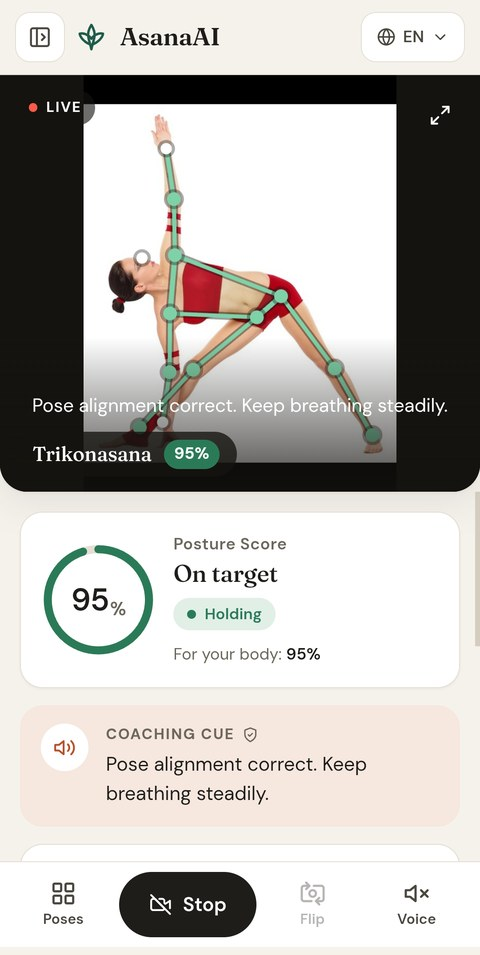
\includegraphics[width=\linewidth]{ui_triangle_en.jpg}\caption{Free mode}\end{subfigure}\hfill
\begin{subfigure}[t]{0.19\textwidth}\centering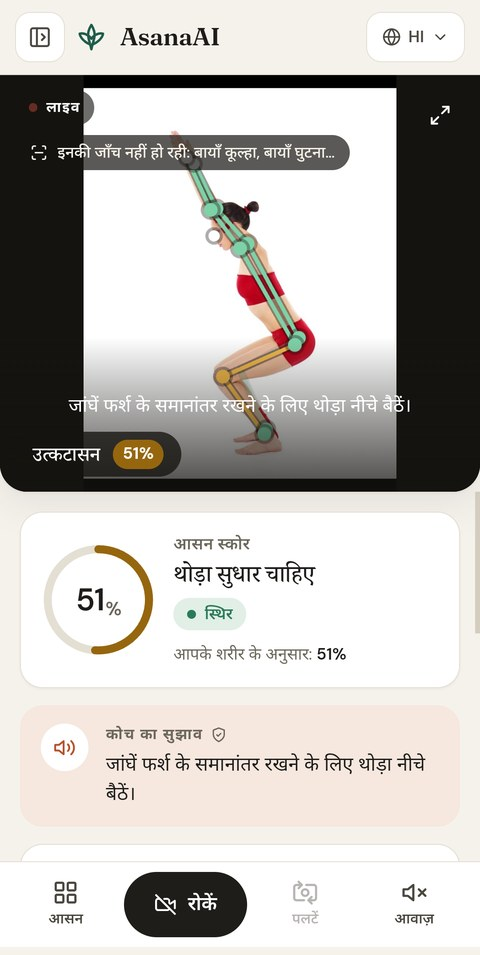
\includegraphics[width=\linewidth]{ui_chair_hi.jpg}\caption{Hindi cue, amber}\end{subfigure}\hfill
\begin{subfigure}[t]{0.19\textwidth}\centering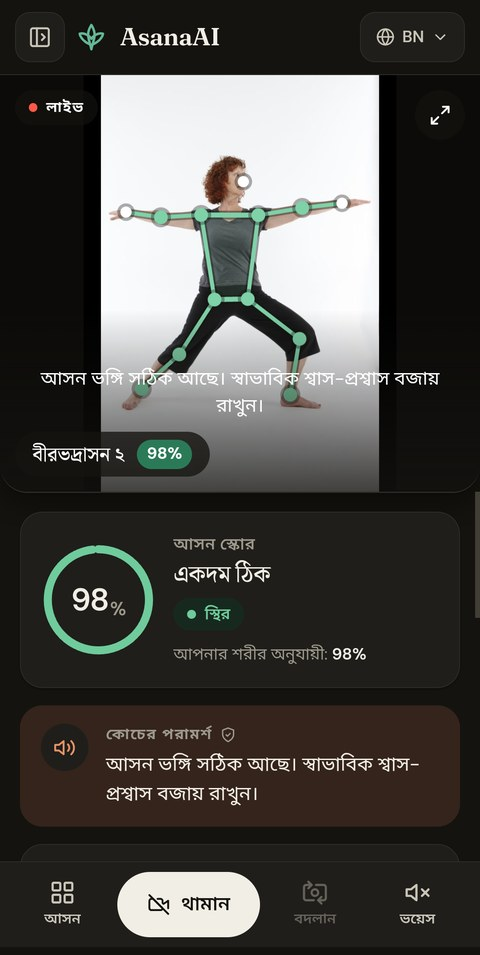
\includegraphics[width=\linewidth]{ui_warrior_bn_dark.jpg}\caption{Bengali, dark theme}\end{subfigure}\hfill
\begin{subfigure}[t]{0.19\textwidth}\centering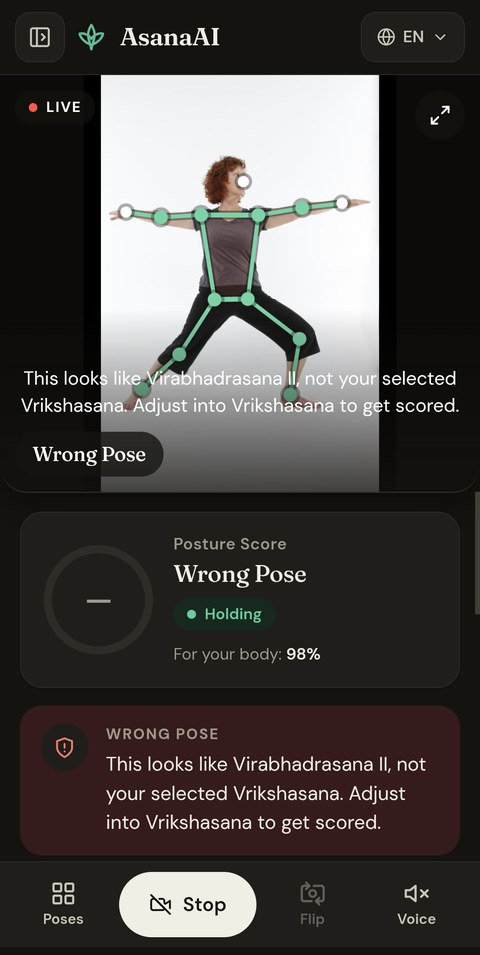
\includegraphics[width=\linewidth]{ui_guided_wrong.jpg}\caption{Guided: wrong pose}\end{subfigure}\hfill
\begin{subfigure}[t]{0.19\textwidth}\centering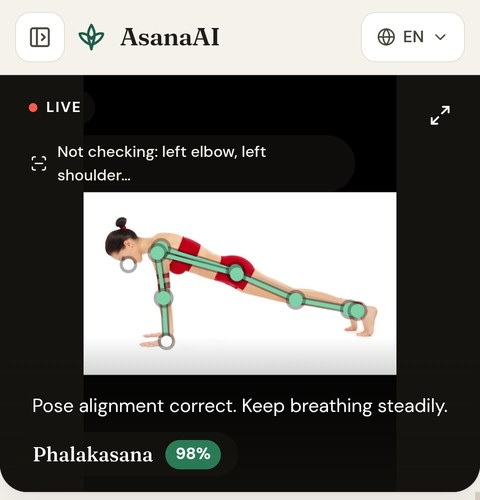
\includegraphics[width=\linewidth]{oc_plank_hidden.jpg}\caption{Hidden joints not judged}\end{subfigure}
\caption{The deployed interface on a POCO M7 Pro, with a credited Wikimedia photo standing in for the camera. (a)~Trikonasana with the posture-score ring and the ``for your body'' personal score. (b)~Utkatasana: the cue in Hindi, a score in amber, and a chip naming the joints not checked. (c)~Virabhadrasana~II, Bengali, dark theme. (d)~Guided mode with Vrikshasana selected while a Warrior~II photo is shown: the score is withheld and the app names the pose it sees. (e)~Plank in guided mode: hidden limbs are drawn faint and are neither scored nor coached. Photos: Kennguru (a, b, e; CC BY 3.0), lululemon athletica (c, d; CC BY 2.0), via Wikimedia Commons.}
\end{figure}

%==========================================================================
\FloatBarrier
\section{Server Architecture}
\subsection{Hosting and process model}
The API is a FastAPI application (\code{backend/app/main.py}) served from a Hugging Face Space. The Space uses the Gradio SDK: its entry point \code{backend/app.py} mounts a small demo page and imports the same FastAPI application, so every \code{/api/*} route is available on the Space URL. At start-up the server downloads the model files from the Hugging Face model repository and caches them; PyTorch is limited to a fixed number of CPU threads. Cross-origin access is restricted to the production web origin and local development origins. The endpoints are stateless: anything that needs history (for example motion) is computed by the client and sent in the request, so the Space can run several workers.

\subsection{Endpoints}
\begin{table}[ht]
\centering\small
\caption{The API (all routes under \code{/api}, JSON).}\label{tab:api}
\begin{tabularx}{\textwidth}{@{}L{5.1cm}L{4.1cm}Y@{}}
\toprule
Route & Request & Response \\ \midrule
\code{POST /analyse\_frame} & \code{angles} (15 floats, required); optional \code{calibration}, \code{motion}, \code{target\_pose}, \code{world\_angles}, \code{orientation} & \code{pose\_id}, \code{correctness\_score}, \code{deviations} (15 joints, degrees), \code{motion\_state}, top-3 \code{candidates}, \code{cascade} info, optional \code{personal\_correctness\_score}, \code{calibrated\_deviations}, \code{guided} \\
\code{POST /analyse\_sequence} & \code{coordinates}: exactly 60 frames $\times$ 99 numbers & \code{sequence\_pose}, \code{confidence}, \code{requires\_static\_fallback}, \code{sequence\_kind} \\
\code{POST /generate\_correction} & \code{pose\_id}, \code{deviations}, \code{language}, \code{attempt} (how many times this cue was already delivered without the joint improving) & \code{correction\_text} (template or screened paraphrase), \code{is\_safe}, \code{target\_joint} \\
\code{POST /occlusion\_recovery} & \code{mp\_landmarks} (33$\times$4), optional \code{cliff\_landmarks} & Optional hook for mesh-based recovery of hidden joints; not used by the deployed app \\
\code{GET /health} & -- & Service status \\ \bottomrule
\end{tabularx}
\end{table}

\subsection{Handling one frame}
\code{analyse\_frame} validates that exactly 15 angles arrived, runs the namer and the gate on the same input tensor (a few milliseconds on a CPU), and passes both outputs to the cascade decision (Section~\ref{sec:cascade}). In the cascade the form score is the gate's correctness logit passed through a sigmoid, and the per-joint deviations are the distances outside the pose's angle bands; the deviation head's output (multiplied by 180 and clipped to $[0^\circ,180^\circ]$) is used only on the fallback path. If the request carried a calibration profile, a second, personalised score is computed (Section~\ref{sec:calib}); if it carried a target pose, a \code{guided} block scores the body against that pose. \code{motion\_state} (``holding'', ``transitioning'', ``unrecognized'') comes from the angular speed the client measured over the last 1.5\,s: you do not correct someone mid-movement, but you do tell them when a held posture is not recognised.

\subsection{Handling one window}
\code{analyse\_sequence} requires exactly $60\times99$ numbers. The window is translated so the pelvis (midpoint of landmarks 23 and 24) is the origin, divided by the hip width, and passed to the ST-GCN; the softmax top class and its confidence are returned. The answer is flagged \code{requires\_static\_fallback} when the class is \code{transition/unknown} or the confidence is below 0.70 (0.55 for child's pose); the app then shows ``static check'' and relies on the per-frame result alone.

\subsection{Configuration and rollback}
\begin{table}[ht]
\centering\small
\caption{Server switches (environment variables, set as Space variables). Defaults equal the production setting.}\label{tab:switches}
\begin{tabularx}{\textwidth}{@{}L{4.6cm}L{4.4cm}Y@{}}
\toprule
Variable & Default & Effect \\ \midrule
\code{ENABLE\_POSE\_CASCADE} & \code{1} & \code{0} reverts to the original single-model path without a redeploy \\
\code{GATE\_MODEL\_FILE}, \code{GATE\_ENCODER\_FILE} & \code{mlp\_3head\_gate\_v1.pth} and its encoder & Gate checkpoint; if it cannot be loaded the endpoint answers with the original path and reports the reason in \code{cascade.reason} \\
\code{STGCN\_MODEL\_FILE}, \code{STGCN\_ENCODER\_FILE} & \code{stgcn\_target\_v1.pth} and its encoder & Sequence checkpoint; older checkpoints stay in the repository and can be selected here \\
\code{GATE\_REPO} & \code{Arko007/}\allowbreak\code{yoga-posture-models} & Where the gate is downloaded from (the namer and the sequence model use the \code{HF\_REPO} setting in \code{config.py}, the same repository) \\ \bottomrule
\end{tabularx}
\end{table}

%==========================================================================
\FloatBarrier
\section{The Models}
\subsection{What goes into each model}
\begin{itemize}
\item The two \textbf{pose MLPs} (namer and gate) read the \emph{15 planar joint angles} of one frame (Table~\ref{tab:features}).
\item The \textbf{ST-GCN} reads a \emph{window of 60 frames $\times$ 33 joints $\times$ $(x,y,z)$}, pelvis-centred and divided by hip width, so it is independent of where the person stands and how far from the camera.
\end{itemize}
This division is deliberate: the MLPs are a single-frame form check from view-independent angles; the ST-GCN adds the skeleton's graph structure, the temporal flow and depth.

\subsection{The 3-head residual MLP}
Both the namer and the gate are the same architecture, \code{Yoga3HeadMLP} (\code{backend/app/models/mlp.py}). A shared trunk feeds three heads, so one forward pass answers ``which pose, how well, which joints''.

\begin{figure}[ht]
\centering
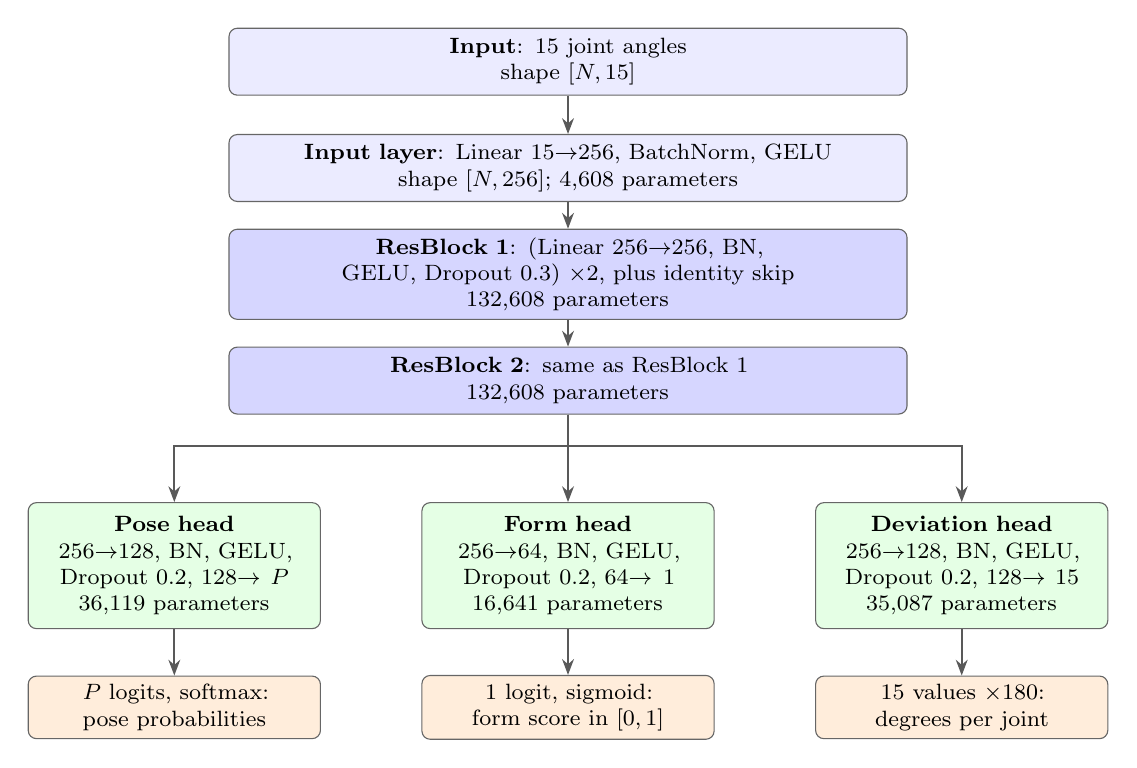
\begin{tikzpicture}[x=1cm,y=1cm]
\node[bx,text width=8.4cm,minimum height=0.85cm] (in) at (0,0) {\textbf{Input}: 15 joint angles\\ shape $[N,15]$};
\node[bx,text width=8.4cm,minimum height=0.85cm] (l1) at (0,-1.35) {\textbf{Input layer}: Linear 15$\to$256, BatchNorm, GELU\\ shape $[N,256]$; 4,608 parameters};
\node[bx,fill=blue!16,text width=8.4cm,minimum height=0.85cm] (r1) at (0,-2.7) {\textbf{ResBlock 1}: (Linear 256$\to$256, BN, GELU, Dropout 0.3) $\times2$, plus identity skip\\ 132,608 parameters};
\node[bx,fill=blue!16,text width=8.4cm,minimum height=0.85cm] (r2) at (0,-4.05) {\textbf{ResBlock 2}: same as ResBlock 1\\ 132,608 parameters};
\node[gx,text width=3.5cm,minimum height=1.6cm] (h1) at (-5.0,-6.4) {\textbf{Pose head}\\ 256$\to$128, BN, GELU, Dropout 0.2, 128$\to P$\\ 36,119 parameters};
\node[gx,text width=3.5cm,minimum height=1.6cm] (h2) at (0,-6.4) {\textbf{Form head}\\ 256$\to$64, BN, GELU, Dropout 0.2, 64$\to1$\\ 16,641 parameters};
\node[gx,text width=3.5cm,minimum height=1.6cm] (h3) at (5.0,-6.4) {\textbf{Deviation head}\\ 256$\to$128, BN, GELU, Dropout 0.2, 128$\to15$\\ 35,087 parameters};
\node[ox,text width=3.5cm] (o1) at (-5.0,-8.2) {$P$ logits, softmax:\\ pose probabilities};
\node[ox,text width=3.5cm] (o2) at (0,-8.2) {1 logit, sigmoid:\\ form score in $[0,1]$};
\node[ox,text width=3.5cm] (o3) at (5.0,-8.2) {15 values $\times180$:\\ degrees per joint};
\draw[ar] (in)--(l1); \draw[ar] (l1)--(r1); \draw[ar] (r1)--(r2);
\draw[ar] (r2.south) -- ++(0,-0.4) -| (h1.north);
\draw[ar] (r2.south) -- (h2.north);
\draw[ar] (r2.south) -- ++(0,-0.4) -| (h3.north);
\foreach \k in {1,2,3}{\draw[ar] (h\k)--(o\k);}
\end{tikzpicture}
\caption{The 3-head residual MLP. $P=23$ pose classes in both deployed models; 357,671 parameters in total (counted from the model definition). Shapes are for a batch of $N$ frames.}
\label{fig:mlp}
\end{figure}

\begin{itemize}
\item \textbf{Pose head}: the class scores. The class list comes from the model's encoder file; classes named \code{imperfect\_<pose>} are summed onto their base pose at serving time.
\item \textbf{Form head}: one logit, trained as a ``correct versus deliberately imperfect or non-pose frame'' probability; a sigmoid turns it into the form score.
\item \textbf{Deviation head}: how far each of the 15 joints is from correct, in units of $1/180$.
\end{itemize}
Residual connections let the 256-wide trunk train stably; batch normalisation and dropout regularise a model that is small enough to run in a few milliseconds.

\subsection{The cascade: one model names, another vetoes}\label{sec:cascade}
Two checkpoints of this architecture are used together. The \textbf{namer} is the pose model whose top class is the answer. The \textbf{gate} was trained with an explicit ``none of our poses'' class (\code{transition/unknown}); it answers the question ``is this one of my poses at all?'' and supplies the form score. The rule engine does not override either model on the pose \emph{name}; it only supplies per-joint deviations.

\begin{figure}[ht]
\centering
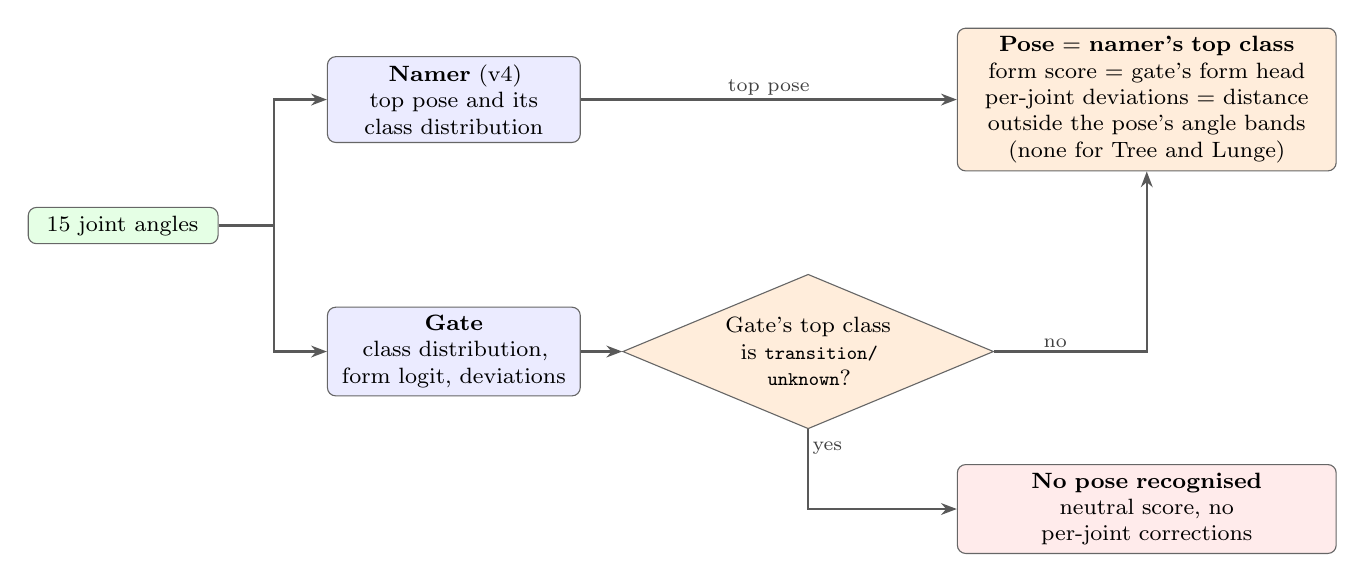
\begin{tikzpicture}[x=1cm,y=1cm]
\node[gx,text width=2.2cm] (ang) at (0,0) {15 joint angles};
\node[bx,text width=3.0cm] (nm) at (4.2,1.6) {\textbf{Namer} (\vfour)\\ top pose and its class distribution};
\node[bx,text width=3.0cm] (gt) at (4.2,-1.6) {\textbf{Gate}\\ class distribution, form logit, deviations};
\node[dm,text width=2.4cm] (d1) at (8.7,-1.6) {Gate's top class is \texttt{\scriptsize transition/ unknown}?};
\node[ox,text width=4.6cm] (yes) at (13.0,1.6) {\textbf{Pose $=$ namer's top class}\\ form score $=$ gate's form head\\ per-joint deviations $=$ distance outside the pose's angle bands (none for Tree and Lunge)};
\node[rx,text width=4.6cm] (no) at (13.0,-3.6) {\textbf{No pose recognised}\\ neutral score, no per-joint corrections};
\draw[ar] (ang.east) -- ++(0.7,0) |- (nm.west);
\draw[ar] (ang.east) -- ++(0.7,0) |- (gt.west);
\draw[ar] (gt.east) -- (d1.west);
\draw[ar] (nm.east) -- node[above,lb]{top pose} (yes.west |- nm.east);
\draw[ar] (d1.east) -| node[above,lb,pos=0.2]{no} (yes.south);
\draw[ar] (d1.south) |- node[right,lb,pos=0.12]{yes} (no.west);
\end{tikzpicture}
\caption{The per-frame decision. The namer and the gate see the same 15 angles. The answer is the namer's pose unless the gate says the frame is not one of the app's poses.}
\label{fig:cascade}
\end{figure}

In code (\code{backend/app/services/cascade.py}, pure logic without PyTorch, so it is unit-tested directly):
\begin{lstlisting}
gate_pose = argmax(collapse(gate_distribution))
gated     = (gate_pose == "transition/unknown")
pose      = "transition/unknown" if gated else sanitize(namer_pose)
if pose == "transition/unknown":
    return no_pose_result                      # neutral score, zero deviations
form      = sigmoid(gate_correctness_logit)    # form score from the gate
if pose has angle bands:   deviations = distance_outside_bands(pose, angles)
else:                      deviations = zeros  # Tree and Lunge: no per-joint claims
\end{lstlisting}
The response also reports the namer's top three candidates and the gate's view (\code{cascade}: \code{active}, \code{gated}, \code{gate\_pose}, \code{gate\_other\_prob}, and the sources of the score and deviations), so a client can show ambiguity honestly. If the gate cannot be loaded, or the switch is off, the endpoint falls back to the original path (the namer plus the rule engine's vote) and says so in the response.

\subsection{The rule engine and per-joint corrections}
Each pose has a table of reference angle bands, for example for Downward Dog: knee in $[110^\circ,180^\circ]$, shoulder in $[95^\circ,180^\circ]$, hip in $[20^\circ,140^\circ]$. The \emph{deviation} of a joint is the distance in degrees outside its band (zero if inside); the rule score is $1-\bar d/45^\circ$ clipped to $[0,1]$. The vocabulary has 19 poses (mountain, upward salute, downward dog, plank, cobra, child, seated staff, seated easy, tree, warrior I, warrior II, lunge, standing forward fold, halfway lift, chair, table top, standing, triangle, corpse); 17 have bands. Tree and Lunge have no bands, so the system makes no per-joint claim for them and draws neutral limbs. Because the learned deviation head is the weakest of the three, joint-level corrections and limb colours come from the bands wherever they exist. The same table is implemented in Python (server) and TypeScript (basic mode).

\subsection{The ST-GCN sequence model}\label{sec:stgcn}
\paragraph{Why a graph network.} A skeleton is not a grid: its joints are connected in a fixed way. A spatial-temporal graph convolutional network (ST-GCN) treats the 33 MediaPipe landmarks as the nodes of a graph whose edges are the bones, and slides a temporal filter over 60 frames, so each joint's features are mixed with its anatomical neighbours and with its own recent past.

\begin{figure}[ht]
\centering
\begin{subfigure}[t]{0.38\textwidth}\centering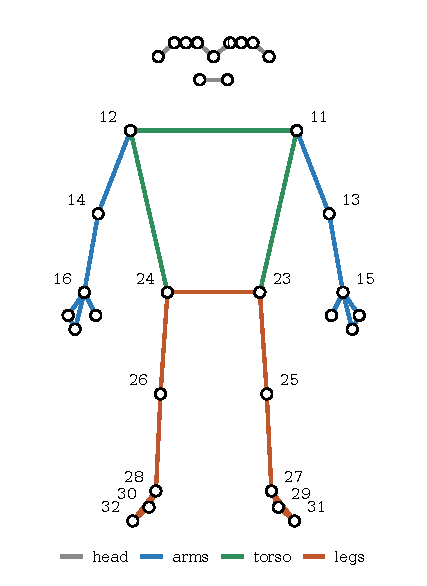
\includegraphics[width=\linewidth]{fig_skeleton_graph.pdf}\caption{The graph: 33 nodes, 35 bones}\end{subfigure}\hspace{0.06\textwidth}
\begin{subfigure}[t]{0.5\textwidth}\centering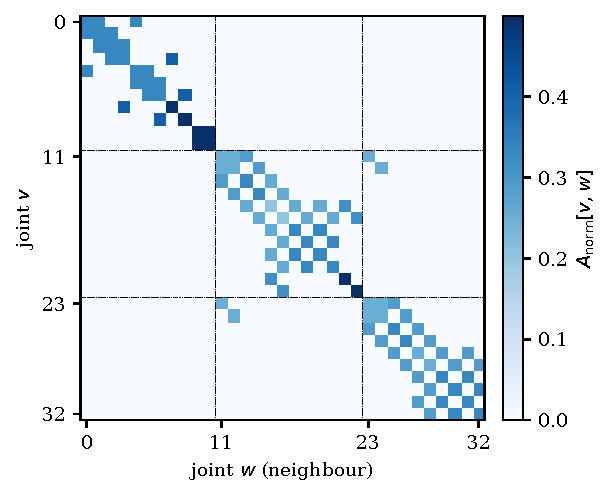
\includegraphics[width=\linewidth]{fig_adjacency.pdf}\caption{$A_{\mathrm{norm}}$ ($33\times33$, 103 non-zero entries)}\end{subfigure}
\caption{The skeleton graph used by the ST-GCN (drawn from the model's own definition). (a)~MediaPipe landmarks and the 35 skeletal edges (numbers are landmark indices; subject's left is on the right). (b)~The symmetric-normalised adjacency $A_{\mathrm{norm}}=D^{-1/2}(A+I)D^{-1/2}$: block structure shows the head, the arms and torso, and the legs; the diagonal is the self-loop.}
\end{figure}

\paragraph{One block.} A block (Figure~\ref{fig:block}) applies (i) a $1\times1$ convolution that projects each joint's channels, (ii) a graph aggregation $\mathbf{Y}[c,v,t]=\sum_{w}A_{\mathrm{norm}}[v,w]\,\mathbf{X}[c,w,t]$ implemented as \code{einsum('vw,ncwt->ncvt')}, (iii) GELU, (iv) a temporal convolution with a $9\times1$ kernel over the 60 frames for each joint independently, followed by batch normalisation and dropout, and (v) a residual connection, with a $1\times1$ convolution and batch normalisation on the skip path when the channel count changes.

\begin{figure}[ht]
\centering
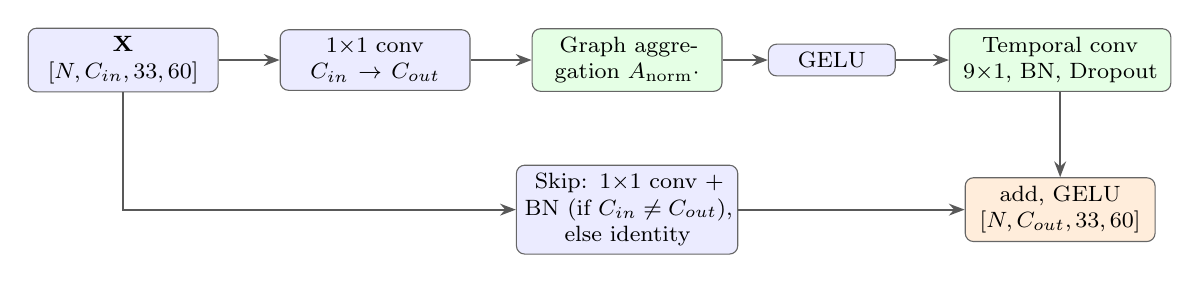
\begin{tikzpicture}[x=1cm,y=1cm]
\node[bx,text width=2.2cm] (x) at (0,0) {$\mathbf{X}$\\ $[N,C_{in},33,60]$};
\node[bx,text width=2.2cm] (p) at (3.2,0) {$1{\times}1$ conv\\ $C_{in}\to C_{out}$};
\node[gx,text width=2.2cm] (g) at (6.4,0) {Graph aggregation $A_{\mathrm{norm}}\cdot$};
\node[bx,text width=1.4cm] (ge) at (9.0,0) {GELU};
\node[gx,text width=2.6cm] (t) at (11.9,0) {Temporal conv $9{\times}1$, BN, Dropout};
\node[bx,text width=2.6cm] (s) at (6.4,-1.9) {Skip: $1{\times}1$ conv + BN (if $C_{in}\ne C_{out}$), else identity};
\node[ox,text width=2.2cm] (o) at (11.9,-1.9) {add, GELU\\ $[N,C_{out},33,60]$};
\foreach \a/\b in {x/p,p/g,g/ge,ge/t}{\draw[ar] (\a)--(\b);}
\draw[ar] (x.south) |- (s.west);
\draw[ar] (s.east) -- (o.west);
\draw[ar] (t.south) -- (o.north);
\end{tikzpicture}
\caption{Inside one ST-GCN block. The graph step mixes each joint with its neighbours; the temporal step mixes each joint with its neighbours in time.}
\label{fig:block}
\end{figure}

\paragraph{The whole network.} Three blocks raise the channel count $3\to64\to128\to256$ (no temporal striding, so all 60 frames are kept), the features are averaged over all joints and frames, and a small head produces the class scores.

\begin{figure}[ht]
\centering
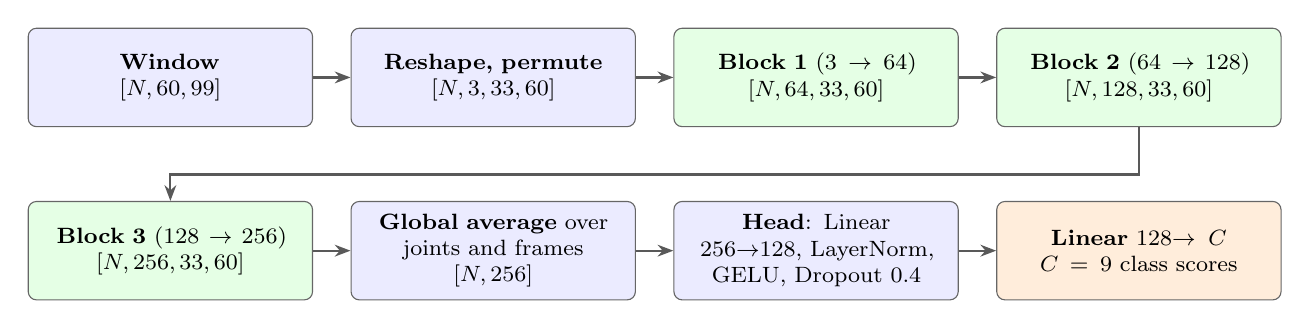
\begin{tikzpicture}[x=1cm,y=1cm]
\tikzset{nd/.style={text width=3.4cm,minimum height=1.25cm}}
\node[bx,nd] (a) at (0,0) {\textbf{Window}\\ $[N,60,99]$};
\node[bx,nd] (b) at (4.1,0) {\textbf{Reshape, permute}\\ $[N,3,33,60]$};
\node[gx,nd] (c) at (8.2,0) {\textbf{Block 1} ($3\to64$)\\ $[N,64,33,60]$};
\node[gx,nd] (d) at (12.3,0) {\textbf{Block 2} ($64\to128$)\\ $[N,128,33,60]$};
\node[gx,nd] (e) at (0,-2.2) {\textbf{Block 3} ($128\to256$)\\ $[N,256,33,60]$};
\node[bx,nd] (f) at (4.1,-2.2) {\textbf{Global average} over joints and frames\\ $[N,256]$};
\node[bx,nd] (g) at (8.2,-2.2) {\textbf{Head}: Linear 256$\to$128, LayerNorm, GELU, Dropout 0.4};
\node[ox,nd] (h) at (12.3,-2.2) {\textbf{Linear} 128$\to C$\\ $C=9$ class scores};
\foreach \s/\t in {a/b,b/c,c/d,e/f,f/g,g/h}{\draw[ar] (\s)--(\t);}
\draw[ar] (d.south) -- ++(0,-0.6) -| (e.north);
\end{tikzpicture}
\caption{ST-GCN data flow with tensor shapes, read left to right and then continued on the second row. $N$ is the batch size; the input has 60 frames, 33 joints and three coordinates per joint.}
\end{figure}

\begin{table}[ht]
\centering\small
\caption{ST-GCN parameter budget (counted from the model definition; $C=9$).}\label{tab:stgcnparams}
\begin{tabular}{@{}lrrrr@{}}
\toprule
Stage & Graph conv & Temporal conv & Skip & Total \\ \midrule
Block 1 ($3\to64$) & 256 & 37,056 & 384 & 37,696 \\
Block 2 ($64\to128$) & 8,320 & 147,840 & 8,576 & 164,736 \\
Block 3 ($128\to256$) & 33,024 & 590,592 & 33,536 & 657,152 \\
Head (256$\to$128$\to9$) & \multicolumn{3}{c}{} & 34,313 \\ \midrule
\textbf{Total} & \multicolumn{3}{c}{} & \textbf{893,897} \\ \bottomrule
\end{tabular}
\end{table}

\paragraph{Output vocabulary and role.} The deployed network (\code{stgcn\_target\_v1}) has 9 classes: child's pose, corpse, downward dog, plank, seated easy, tree, triangle, warrior II, and \code{transition/unknown}. It acts as a second opinion over the last 2.4\,s (the ``flow check'') and is shown only when confident; it never overrides the per-frame pose. The Python class is called \code{YogaSequenceLSTM} for checkpoint compatibility only; it contains no recurrent layer.

\subsection{How the outputs reach the screen}
\begin{table}[H]
\centering\small
\caption{Which component produces each thing the user sees.}\label{tab:fusion}
\begin{tabularx}{\textwidth}{@{}L{4.2cm}Y@{}}
\toprule
On screen & Produced by \\ \midrule
Pose name & Namer, unless the gate vetoes (then ``not recognised''); in basic mode, the rule engine \\
Posture score (ring) & Gate's form head; ``for your body'' score from the personal calibration \\
Limb colours and per-joint cue & Rule-engine angle bands (none for Tree and Lunge); hidden joints excluded \\
Flow check / static check & ST-GCN if its confidence passes the threshold, otherwise ``static check'' \\
Coaching sentence & Template $\to$ optional language-model paraphrase $\to$ safety screen \\
Wrong-pose card (guided mode) & Detected pose differs from the chosen target pose \\ \bottomrule
\end{tabularx}
\end{table}

%==========================================================================
\FloatBarrier
\section{Calibration, Visibility and Coaching}
\subsection{Personal range-of-motion calibration}\label{sec:calib}
Bodies differ, so a joint inside its owner's comfortable range is ``different'', not ``wrong''. At camera start the app can run a 15-second calibration while the user stands comfortably in view. For each of the 15 joints the profile stores the observed minimum and maximum widened by $15^\circ$ (clamped to $[0^\circ,180^\circ]$) and the mean as the resting angle; a profile with fewer than 20 frames is discarded. The profile lives only in the browser's local storage and is sent as numbers with each request. On the server a joint inside its personal range has its deviation set to zero and a second, personalised score is returned; it is never lower than the universal score and equals it when nothing is forgiven.

\begin{figure}[ht]
\centering
\begin{subfigure}[t]{0.2\textwidth}\centering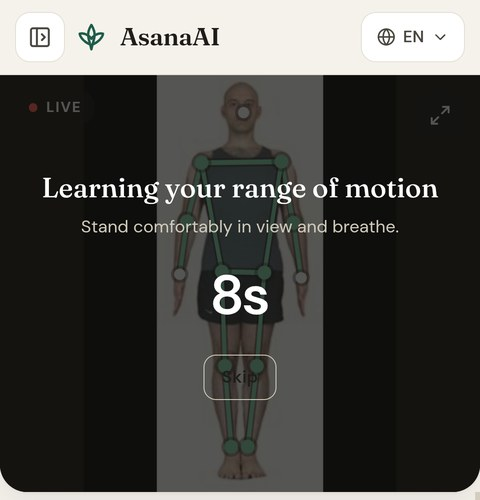
\includegraphics[width=\linewidth]{cal_countdown.jpg}\caption{Countdown}\end{subfigure}\hspace{0.05\textwidth}
\begin{subfigure}[t]{0.2\textwidth}\centering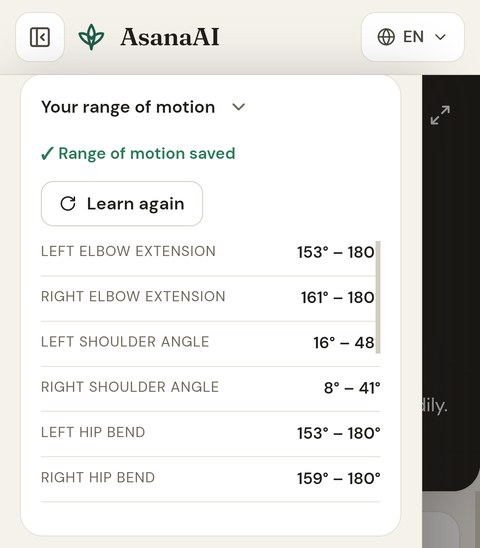
\includegraphics[width=\linewidth]{cal_range.jpg}\caption{Saved ranges}\end{subfigure}
\caption{Calibration screens: (a)~15-second capture; (b)~the learned per-joint ranges, stored on the device.}
\end{figure}

\subsection{Visibility-aware scoring}
Instead of guessing hidden joints, the system abstains: landmarks with low smoothed visibility are excluded from the score, from the per-joint cue and from the limb colouring, and the interface lists what is not being checked. (A server hook for mesh-based recovery of hidden joints exists in the code but is not used by the deployed app, because it would need the camera image, which never leaves the device.)

\subsection{Safe, multilingual coaching}
\begin{figure}[ht]
\centering
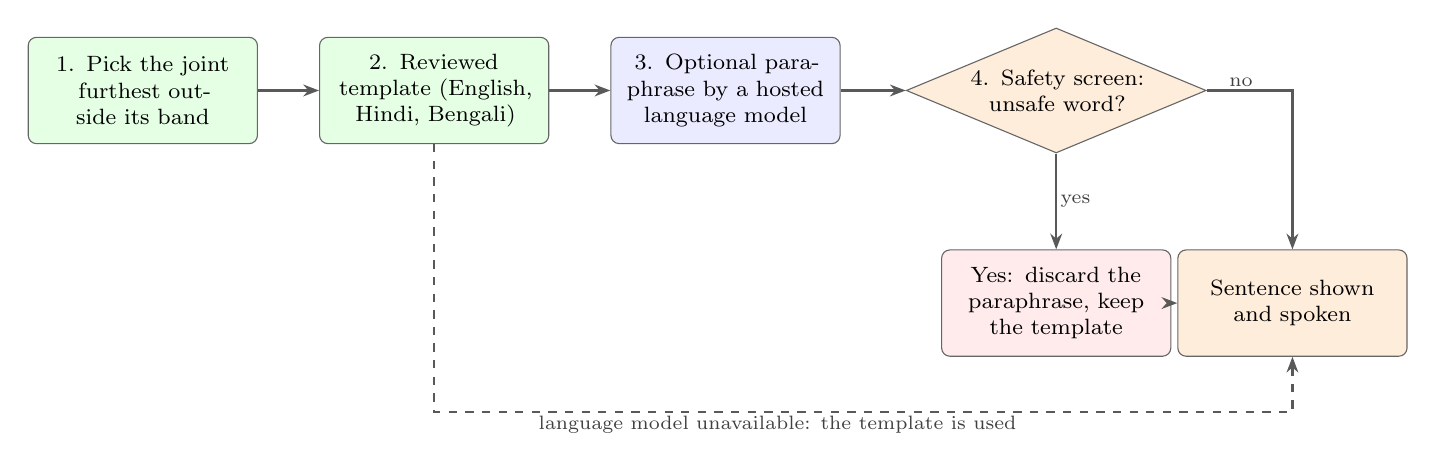
\begin{tikzpicture}[x=1cm,y=1cm]
\tikzset{nd/.style={text width=2.7cm,minimum height=1.35cm}}
\node[gx,nd] (a) at (0,0) {1. Pick the joint furthest outside its band};
\node[gx,nd] (b) at (3.7,0) {2. Reviewed template (English, Hindi, Bengali)};
\node[bx,nd] (c) at (7.4,0) {3. Optional paraphrase by a hosted language model};
\node[dm,text width=2.3cm] (d) at (11.6,0) {4. Safety screen: unsafe word?};
\node[rx,nd] (k) at (11.6,-2.7) {Yes: discard the paraphrase, keep the template};
\node[ox,nd] (f) at (14.6,-2.7) {Sentence shown and spoken};
\foreach \s/\t in {a/b,b/c}{\draw[ar] (\s)--(\t);}
\draw[ar] (c)--(d.west);
\draw[ar] (d.south)--node[right,lb]{yes}(k.north);
\draw[ar] (k.east)--(f.west);
\draw[ar] (d.east) -| node[above,lb,pos=0.2]{no} (f.north);
\draw[ar,dashed] (b.south) -- ++(0,-3.4) -| node[below,lb,pos=0.2]{language model unavailable: the template is used} (f.south);
\end{tikzpicture}
\caption{The coaching pipeline. The language model may only rewrite a reviewed sentence; the template is always the fallback.}
\end{figure}
The language model is a 27-billion-parameter Qwen model reached through a hosted API (8\,s timeout, temperature 0.2). The screen discards any paraphrase containing ``push'', ``force'', ``hurt'', ``pain'', ``stretch more'' or ``further''. This English list is applied to every language, because a model can slip an English word into a Hindi or Bengali answer; equivalent Hindi and Bengali word lists, reviewed by a native speaker of both languages, cover the other two languages. Cues escalate on a fixed ladder: the second delivery of a cue that produced no measured improvement adds how many degrees off the user is; from the third time the cue backs off (ease out of the shape and come back only as far as feels comfortable), because a cue that failed twice usually means the range is not available today.

%==========================================================================
\FloatBarrier
\section{Deployment Topology and Operations}
\begin{figure}[ht]
\centering
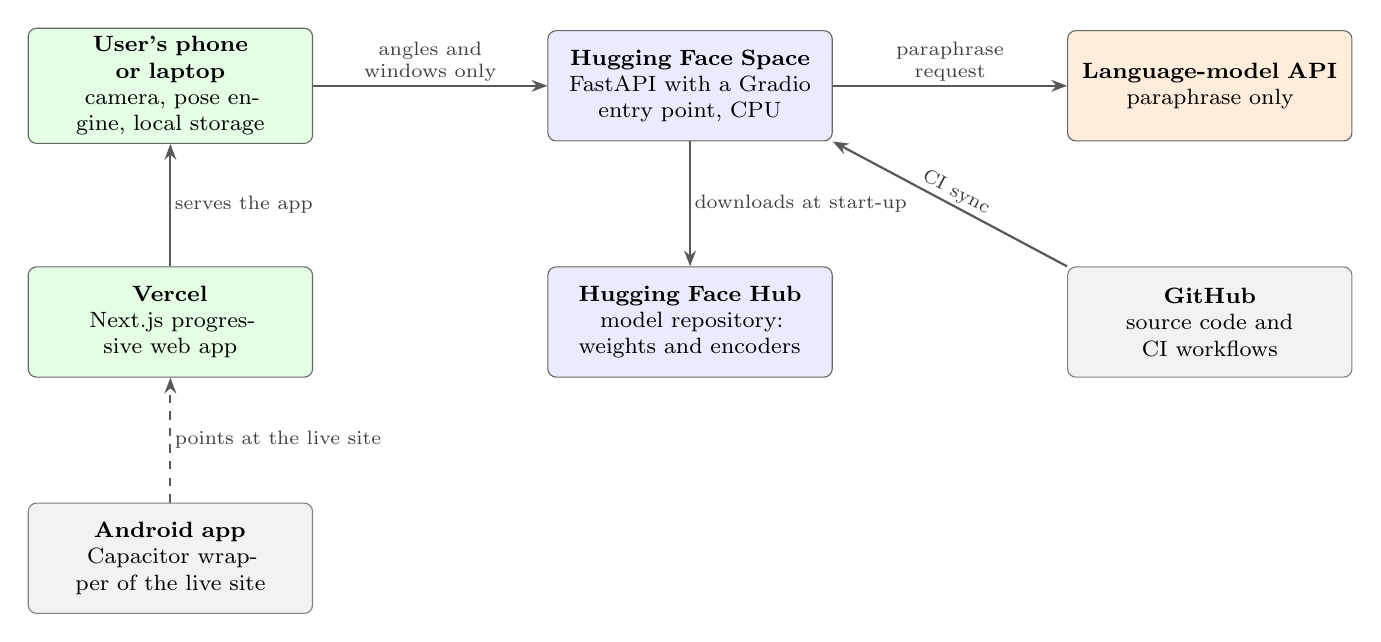
\begin{tikzpicture}[x=1cm,y=1cm]
\tikzset{nd/.style={text width=3.4cm,minimum height=1.4cm}}
\node[gx,nd] (u) at (0,0) {\textbf{User's phone or laptop}\\ camera, pose engine, local storage};
\node[bx,nd] (s) at (6.6,0) {\textbf{Hugging Face Space}\\ FastAPI with a Gradio entry point, CPU};
\node[ox,nd] (l) at (13.2,0) {\textbf{Language-model API}\\ paraphrase only};
\node[gx,nd] (v) at (0,-3.0) {\textbf{Vercel}\\ Next.js progressive web app};
\node[bx,nd] (m) at (6.6,-3.0) {\textbf{Hugging Face Hub}\\ model repository: weights and encoders};
\node[gy,nd] (g) at (13.2,-3.0) {\textbf{GitHub}\\ source code and CI workflows};
\node[gy,nd] (a) at (0,-6.0) {\textbf{Android app}\\ Capacitor wrapper of the live site};
\draw[ar] (v)--node[right,lb]{serves the app}(u);
\draw[ar] (u)--node[above,lb,text width=2.3cm,align=center]{angles and windows only}(s);
\draw[ar] (s)--node[right,lb]{downloads at start-up}(m);
\draw[ar] (s)--node[above,lb,text width=2.3cm,align=center]{paraphrase request}(l);
\draw[ar] (g.north west)--node[above,lb,sloped,pos=0.5]{CI sync}(s.south east);
\draw[ar,dashed] (a)--node[right,lb]{points at the live site}(v);
\end{tikzpicture}
\caption{Deployment topology. The only data that go from the device to the server are joint angles and landmark windows; the camera image stays in the browser.}
\end{figure}

\begin{itemize}
\item \textbf{Web.} The Next.js app is hosted on Vercel and works as a progressive web app: the pose-engine files are cached after the first visit so it also starts offline.
\item \textbf{API.} A GitHub Actions workflow pushes the backend to the Hugging Face Space whenever \code{backend/**}, \code{README.md} or the workflow itself changes. Changes to documents or training scripts do not redeploy it.
\item \textbf{Android.} A workflow builds a Capacitor debug APK; it is configured in server mode, so it simply points at the live web app. A separate Expo/React Native companion app lives in \code{mobile/}.
\item \textbf{Weights.} Checkpoints are never overwritten: a new model is added under a new file name, and the active one is selected by a variable, so rolling back is a configuration change.
\item \textbf{Cost and footprint.} The server runs on a CPU Space; with all three networks loaded it needs about 324\,MB of memory, and server compute is roughly 7 to 9\,ms per frame request.
\end{itemize}

%==========================================================================
\section{How the Models Are Produced}
\begin{figure}[ht]
\centering
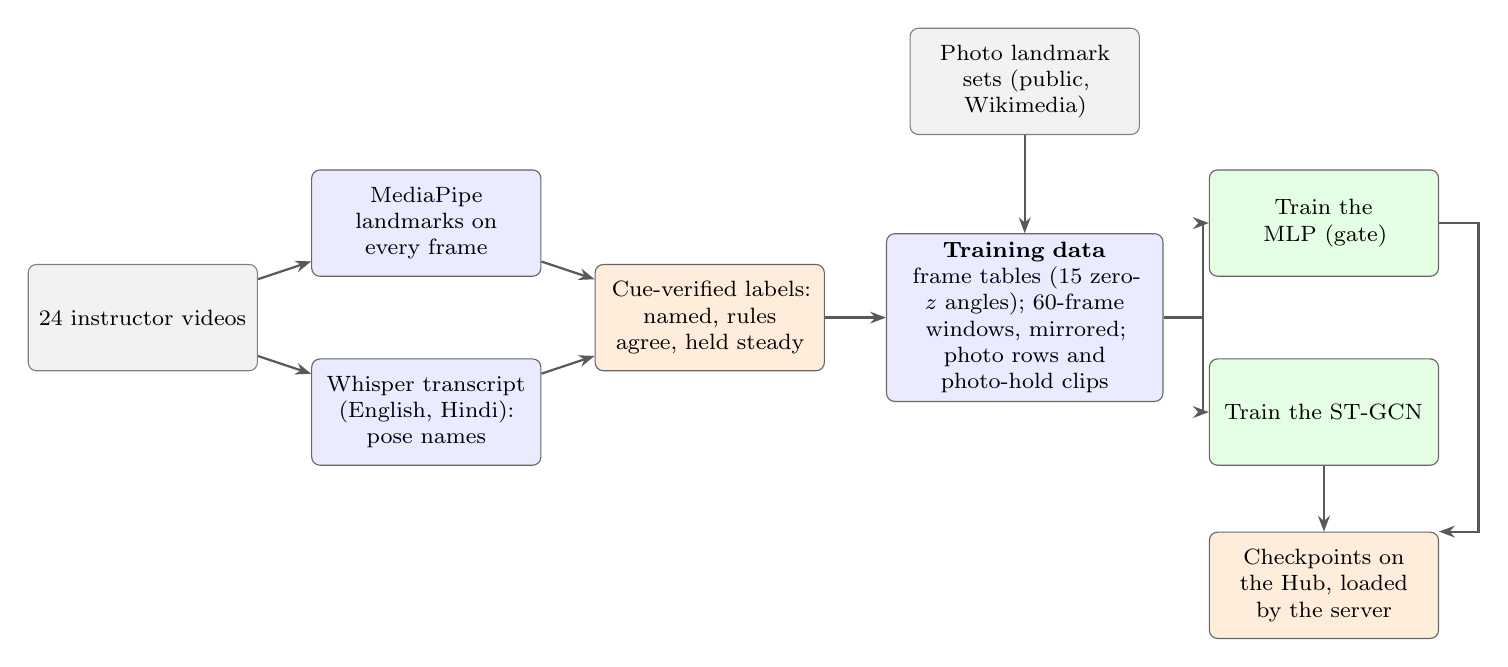
\begin{tikzpicture}[x=1cm,y=1cm]
\tikzset{nd/.style={text width=2.7cm,minimum height=1.35cm}}
\node[gy,nd] (v) at (0,0) {24 instructor videos};
\node[bx,nd] (mp) at (3.6,1.2) {MediaPipe landmarks on every frame};
\node[bx,nd] (wh) at (3.6,-1.2) {Whisper transcript (English, Hindi): pose names};
\node[ox,nd] (lab) at (7.2,0) {Cue-verified labels: named, rules agree, held steady};
\node[bx,text width=3.3cm,minimum height=1.9cm] (dat) at (11.2,0) {\textbf{Training data}\\ frame tables (15 zero-$z$ angles); 60-frame windows, mirrored; photo rows and photo-hold clips};
\node[gy,nd] (ph) at (11.2,3.0) {Photo landmark sets (public, Wikimedia)};
\node[gx,nd] (tr) at (15.0,1.2) {Train the MLP (gate)};
\node[gx,nd] (ts) at (15.0,-1.2) {Train the ST-GCN};
\node[ox,nd] (hub) at (15.0,-3.4) {Checkpoints on the Hub, loaded by the server};
\draw[ar] (v)--(mp); \draw[ar] (v)--(wh); \draw[ar] (mp)--(lab); \draw[ar] (wh)--(lab);
\draw[ar] (lab)--(dat); \draw[ar] (ph)--(dat);
\draw[ar] (dat.east)--++(0.5,0)|-(tr.west); \draw[ar] (dat.east)--++(0.5,0)|-(ts.west);
\draw[ar] (tr.east)--++(0.5,0)|-($(hub.north east)+(0,0.0)$); \draw[ar] (ts.south)--(hub.north);
\end{tikzpicture}
\caption{The model production pipeline. Video frames are labelled only where three independent sources agree; photos add variety that 24 videos cannot. The namer is an earlier checkpoint trained before the cue-verified labels existed (on a 12-video table plus photos).}
\end{figure}

\begin{table}[ht]
\centering\small
\caption{The three production checkpoints (repository \code{Arko007/yoga-posture-models}).}\label{tab:inventory}
\begin{tabularx}{\textwidth}{@{}L{2.6cm}L{5.6cm}rrY@{}}
\toprule
Role & Weights & Parameters & Size & Output \\ \midrule
Namer & \code{mlp\_3head\_v4\_photos\_x2000.pth} & 357,671 & 1.5\,MB & $P{=}23$ pose scores, form, 15 deviations \\
Gate & \code{mlp\_3head\_gate\_v1.pth} & 357,671 & 1.5\,MB & $P{=}23$ pose scores (with ``none of mine''), form, 15 deviations \\
Sequence model & \code{stgcn\_target\_v1.pth} & 893,897 & 3.6\,MB & 9 classes \\ \bottomrule
\end{tabularx}
\end{table}
Each checkpoint is accompanied by an encoder file (\code{.npy}) holding the class names in output order. The training data are published as the Yoga-1M dataset (\url{https://huggingface.co/datasets/Arko007/Yoga-1M}) and the weights as \url{https://huggingface.co/Arko007/yoga-posture-models}; both have a card describing exactly which data trained which model.

%==========================================================================
\needspace{10\baselineskip}
\section{Repository Map}
\begin{table}[H]
\centering\small
\caption{Repository layout (\code{github.com/Anamitra-Sarkar/yoga-posture-correction-system}).}\label{tab:repo}
\begin{tabularx}{\textwidth}{@{}L{5.6cm}Y@{}}
\toprule
Path & Contents \\ \midrule
\code{frontend/src/} (\code{pages}, \code{hooks}, \code{utils}) & The web app: practice screen and landing page; the pipeline hook (\code{useYogaPipeline}); geometry, visibility, sequence buffer, CPU pose engine, offline coach \\
\code{frontend/android/}, \code{mobile/} & Capacitor Android project; Expo companion app \\
\code{backend/app/main.py}, \code{routers/} & FastAPI app and the \code{/api} routes \\
\code{backend/app/models/} & \code{mlp.py} (3-head ResMLP), \code{sequence.py} (ST-GCN) \\
\code{backend/app/services/} & \code{cascade.py} (decision logic), \code{hf\_loader.py} (weights), \code{correction.py} (coaching), \code{occlusion.py} \\
\code{backend/app/utils/} & \code{geometry.py} (angles, window normalisation), \code{rules\_classifier.py} (angle bands, rule engine) \\
\code{backend/tests/} & Unit and endpoint tests \\
\code{modal/}, \code{planning/} & Data preparation and training scripts, Kaggle kernels \\
\code{docs/} & Cascade, sequence-model and benchmark notes; this document \\
\code{paper/}, \code{report/} & Research paper and project report (LaTeX) \\
\code{.github/workflows/} & Space sync and Android build \\ \bottomrule
\end{tabularx}
\end{table}

\end{document}
